% REV01 Sun 27 Jun 2021 13:58:57 WIB
% START Tue 04 May 2021 13:55:16 WIB

\chapter{TWO PLACES VACATED}

Set down by the omnibus at the corner of Saint Mary Axe, and trusting
to her feet and her crutch-stick within its precincts, the dolls’
dressmaker proceeded to the place of business of Pubsey and Co. All
there was sunny and quiet externally, and shady and quiet internally.
Hiding herself in the entry outside the glass door, she could see from
that post of observation the old man in his spectacles sitting writing
at his desk.

‘Boh!’ cried the dressmaker, popping in her head at the glass-door. ‘Mr
Wolf at home?’

The old man took his glasses off, and mildly laid them down beside him.
‘Ah Jenny, is it you? I thought you had given me up.’

‘And so I had given up the treacherous wolf of the forest,’ she replied;
‘but, godmother, it strikes me you have come back. I am not quite sure,
because the wolf and you change forms. I want to ask you a question or
two, to find out whether you are really godmother or really wolf. May
I?’

‘Yes, Jenny, yes.’ But Riah glanced towards the door, as if he thought
his principal might appear there, unseasonably.

‘If you’re afraid of the fox,’ said Miss Jenny, ‘you may dismiss all
present expectations of seeing that animal. HE won’t show himself
abroad, for many a day.’

‘What do you mean, my child?’

‘I mean, godmother,’ replied Miss Wren, sitting down beside the Jew,
‘that the fox has caught a famous flogging, and that if his skin and
bones are not tingling, aching, and smarting at this present instant, no
fox did ever tingle, ache, and smart.’ Therewith Miss Jenny related what
had come to pass in the Albany, omitting the few grains of pepper.

‘Now, godmother,’ she went on, ‘I particularly wish to ask you what has
taken place here, since I left the wolf here? Because I have an idea
about the size of a marble, rolling about in my little noddle. First and
foremost, are you Pubsey and Co., or are you either? Upon your solemn
word and honour.’

The old man shook his head.

‘Secondly, isn’t Fledgeby both Pubsey and Co.?’

The old man answered with a reluctant nod.

‘My idea,’ exclaimed Miss Wren, ‘is now about the size of an orange. But
before it gets any bigger, welcome back, dear godmother!’

The little creature folded her arms about the old man’s neck with great
earnestness, and kissed him. ‘I humbly beg your forgiveness, godmother.
I am truly sorry. I ought to have had more faith in you. But what could
I suppose when you said nothing for yourself, you know? I don’t mean to
offer that as a justification, but what could I suppose, when you were a
silent party to all he said? It did look bad; now didn’t it?’

‘It looked so bad, Jenny,’ responded the old man, with gravity, ‘that I
will straightway tell you what an impression it wrought upon me. I was
hateful in mine own eyes. I was hateful to myself, in being so hateful
to the debtor and to you. But more than that, and worse than that,
and to pass out far and broad beyond myself--I reflected that evening,
sitting alone in my garden on the housetop, that I was doing dishonour
to my ancient faith and race. I reflected--clearly reflected for the
first time--that in bending my neck to the yoke I was willing to wear,
I bent the unwilling necks of the whole Jewish people. For it is not, in
Christian countries, with the Jews as with other peoples. Men say, “This
is a bad Greek, but there are good Greeks. This is a bad Turk, but there
are good Turks.” Not so with the Jews. Men find the bad among us easily
enough--among what peoples are the bad not easily found?--but they take
the worst of us as samples of the best; they take the lowest of us as
presentations of the highest; and they say “All Jews are alike.” If,
doing what I was content to do here, because I was grateful for the past
and have small need of money now, I had been a Christian, I could have
done it, compromising no one but my individual self. But doing it as a
Jew, I could not choose but compromise the Jews of all conditions and
all countries. It is a little hard upon us, but it is the truth. I would
that all our people remembered it! Though I have little right to say so,
seeing that it came home so late to me.’

The dolls’ dressmaker sat holding the old man by the hand, and looking
thoughtfully in his face.

‘Thus I reflected, I say, sitting that evening in my garden on the
housetop. And passing the painful scene of that day in review before
me many times, I always saw that the poor gentleman believed the story
readily, because I was one of the Jews--that you believed the story
readily, my child, because I was one of the Jews--that the story itself
first came into the invention of the originator thereof, because I was
one of the Jews. This was the result of my having had you three before
me, face to face, and seeing the thing visibly presented as upon a
theatre. Wherefore I perceived that the obligation was upon me to leave
this service. But Jenny, my dear,’ said Riah, breaking off, ‘I promised
that you should pursue your questions, and I obstruct them.’

‘On the contrary, godmother; my idea is as large now as a pumpkin--and
YOU know what a pumpkin is, don’t you? So you gave notice that you
were going? Does that come next?’ asked Miss Jenny with a look of close
attention.

‘I indited a letter to my master. Yes. To that effect.’

‘And what said Tingling-Tossing-Aching-Screaming-Scratching-Smarter?’
asked Miss Wren with an unspeakable enjoyment in the utterance of those
honourable titles and in the recollection of the pepper.

‘He held me to certain months of servitude, which were his lawful term
of notice. They expire to-morrow. Upon their expiration--not before--I
had meant to set myself right with my Cinderella.’

‘My idea is getting so immense now,’ cried Miss Wren, clasping her
temples, ‘that my head won’t hold it! Listen, godmother; I am going to
expound. Little Eyes (that’s Screaming-Scratching-Smarter) owes you a
heavy grudge for going. Little Eyes casts about how best to pay you off.
Little Eyes thinks of Lizzie. Little Eyes says to himself, “I’ll find
out where he has placed that girl, and I’ll betray his secret because
it’s dear to him.” Perhaps Little Eyes thinks, “I’ll make love to her
myself too;” but that I can’t swear--all the rest I can. So, Little Eyes
comes to me, and I go to Little Eyes. That’s the way of it. And now the
murder’s all out, I’m sorry,’ added the dolls’ dressmaker, rigid from
head to foot with energy as she shook her little fist before her eyes,
‘that I didn’t give him Cayenne pepper and chopped pickled Capsicum!’

This expression of regret being but partially intelligible to Mr Riah,
the old man reverted to the injuries Fledgeby had received, and hinted
at the necessity of his at once going to tend that beaten cur.

‘Godmother, godmother, godmother!’ cried Miss Wren irritably, ‘I really
lose all patience with you. One would think you believed in the Good
Samaritan. How can you be so inconsistent?’

‘Jenny dear,’ began the old man gently, ‘it is the custom of our people
to help--’

‘Oh! Bother your people!’ interposed Miss Wren, with a toss of her head.
‘If your people don’t know better than to go and help Little Eyes, it’s
a pity they ever got out of Egypt. Over and above that,’ she added, ‘he
wouldn’t take your help if you offered it. Too much ashamed. Wants to
keep it close and quiet, and to keep you out of the way.’

They were still debating this point when a shadow darkened the entry,
and the glass door was opened by a messenger who brought a letter
unceremoniously addressed, ‘Riah.’ To which he said there was an answer
wanted.

The letter, which was scrawled in pencil uphill and downhill and round
crooked corners, ran thus:


‘OLD RIAH,

Your accounts being all squared, go. Shut up the place, turn out
directly, and send me the key by bearer. Go. You are an unthankful dog
of a Jew. Get out.

F.’


The dolls’ dressmaker found it delicious to trace the screaming and
smarting of Little Eyes in the distorted writing of this epistle. She
laughed over it and jeered at it in a convenient corner (to the great
astonishment of the messenger) while the old man got his few goods
together in a black bag. That done, the shutters of the upper windows
closed, and the office blind pulled down, they issued forth upon the
steps with the attendant messenger. There, while Miss Jenny held the
bag, the old man locked the house door, and handed over the key to him;
who at once retired with the same.

‘Well, godmother,’ said Miss Wren, as they remained upon the steps
together, looking at one another. ‘And so you’re thrown upon the world!’

‘It would appear so, Jenny, and somewhat suddenly.’

‘Where are you going to seek your fortune?’ asked Miss Wren.

The old man smiled, but looked about him with a look of having lost his
way in life, which did not escape the dolls’ dressmaker.

‘Verily, Jenny,’ said he, ‘the question is to the purpose, and more
easily asked than answered. But as I have experience of the ready
goodwill and good help of those who have given occupation to Lizzie, I
think I will seek them out for myself.’

‘On foot?’ asked Miss Wren, with a chop.

‘Ay!’ said the old man. ‘Have I not my staff?’

It was exactly because he had his staff, and presented so quaint an
aspect, that she mistrusted his making the journey.

‘The best thing you can do,’ said Jenny, ‘for the time being, at all
events, is to come home with me, godmother. Nobody’s there but my bad
child, and Lizzie’s lodging stands empty.’ The old man when satisfied
that no inconvenience could be entailed on any one by his compliance,
readily complied; and the singularly-assorted couple once more went
through the streets together.

Now, the bad child having been strictly charged by his parent to remain
at home in her absence, of course went out; and, being in the very last
stage of mental decrepitude, went out with two objects; firstly,
to establish a claim he conceived himself to have upon any licensed
victualler living, to be supplied with threepennyworth of rum for
nothing; and secondly, to bestow some maudlin remorse on Mr Eugene
Wrayburn, and see what profit came of it. Stumblingly pursuing these
two designs--they both meant rum, the only meaning of which he was
capable--the degraded creature staggered into Covent Garden Market and
there bivouacked, to have an attack of the trembles succeeded by an
attack of the horrors, in a doorway.

This market of Covent Garden was quite out of the creature’s line of
road, but it had the attraction for him which it has for the worst of
the solitary members of the drunken tribe. It may be the companionship
of the nightly stir, or it may be the companionship of the gin and
beer that slop about among carters and hucksters, or it may be the
companionship of the trodden vegetable refuse which is so like their own
dress that perhaps they take the Market for a great wardrobe; but be
it what it may, you shall see no such individual drunkards on doorsteps
anywhere, as there. Of dozing women-drunkards especially, you shall come
upon such specimens there, in the morning sunlight, as you might
seek out of doors in vain through London. Such stale vapid rejected
cabbage-leaf and cabbage-stalk dress, such damaged-orange countenance,
such squashed pulp of humanity, are open to the day nowhere else. So,
the attraction of the Market drew Mr Dolls to it, and he had out his two
fits of trembles and horrors in a doorway on which a woman had had out
her sodden nap a few hours before.

There is a swarm of young savages always flitting about this same place,
creeping off with fragments of orange-chests, and mouldy litter--Heaven
knows into what holes they can convey them, having no home!--whose bare
feet fall with a blunt dull softness on the pavement as the policeman
hunts them, and who are (perhaps for that reason) little heard by
the Powers that be, whereas in top-boots they would make a deafening
clatter. These, delighting in the trembles and the horrors of Mr Dolls,
as in a gratuitous drama, flocked about him in his doorway, butted
at him, leaped at him, and pelted him. Hence, when he came out of
his invalid retirement and shook off that ragged train, he was much
bespattered, and in worse case than ever. But, not yet at his worst;
for, going into a public-house, and being supplied in stress of business
with his rum, and seeking to vanish without payment, he was collared,
searched, found penniless, and admonished not to try that again,
by having a pail of dirty water cast over him. This application
superinduced another fit of the trembles; after which Mr Dolls, as
finding himself in good cue for making a call on a professional friend,
addressed himself to the Temple.

There was nobody at the chambers but Young Blight. That discreet youth,
sensible of a certain incongruity in the association of such a
client with the business that might be coming some day, with the best
intentions temporized with Dolls, and offered a shilling for coach-hire
home. Mr Dolls, accepting the shilling, promptly laid it out in
two threepennyworths of conspiracy against his life, and two
threepennyworths of raging repentance. Returning to the Chambers with
which burden, he was descried coming round into the court, by the wary
young Blight watching from the window: who instantly closed the outer
door, and left the miserable object to expend his fury on the panels.

The more the door resisted him, the more dangerous and imminent became
that bloody conspiracy against his life. Force of police arriving,
he recognized in them the conspirators, and laid about him hoarsely,
fiercely, staringly, convulsively, foamingly. A humble machine, familiar
to the conspirators and called by the expressive name of Stretcher,
being unavoidably sent for, he was rendered a harmless bundle of torn
rags by being strapped down upon it, with voice and consciousness gone
out of him, and life fast going. As this machine was borne out at the
Temple gate by four men, the poor little dolls’ dressmaker and her
Jewish friend were coming up the street.

‘Let us see what it is,’ cried the dressmaker. ‘Let us make haste and
look, godmother.’

The brisk little crutch-stick was but too brisk. ‘O gentlemen,
gentlemen, he belongs to me!’

‘Belongs to you?’ said the head of the party, stopping it.

‘O yes, dear gentlemen, he’s my child, out without leave. My poor bad,
bad boy! and he don’t know me, he don’t know me! O what shall I do,’
cried the little creature, wildly beating her hands together, ‘when my
own child don’t know me!’

The head of the party looked (as well he might) to the old man for
explanation. He whispered, as the dolls’ dressmaker bent over the
exhausted form and vainly tried to extract some sign of recognition from
it: ‘It’s her drunken father.’

As the load was put down in the street, Riah drew the head of the party
aside, and whispered that he thought the man was dying. ‘No, surely
not?’ returned the other. But he became less confident, on looking, and
directed the bearers to ‘bring him to the nearest doctor’s shop.’

Thither he was brought; the window becoming from within, a wall of
faces, deformed into all kinds of shapes through the agency of globular
red bottles, green bottles, blue bottles, and other coloured bottles. A
ghastly light shining upon him that he didn’t need, the beast so furious
but a few minutes gone, was quiet enough now, with a strange mysterious
writing on his face, reflected from one of the great bottles, as if
Death had marked him: ‘Mine.’

The medical testimony was more precise and more to the purpose than it
sometimes is in a Court of Justice. ‘You had better send for something
to cover it. All’s over.’

Therefore, the police sent for something to cover it, and it was covered
and borne through the streets, the people falling away. After it,
went the dolls’ dressmaker, hiding her face in the Jewish skirts, and
clinging to them with one hand, while with the other she plied her
stick. It was carried home, and, by reason that the staircase was very
narrow, it was put down in the parlour--the little working-bench being
set aside to make room for it--and there, in the midst of the dolls with
no speculation in their eyes, lay Mr Dolls with no speculation in his.

Many flaunting dolls had to be gaily dressed, before the money was in
the dressmaker’s pocket to get mourning for Mr Dolls. As the old man,
Riah, sat by, helping her in such small ways as he could, he found it
difficult to make out whether she really did realize that the deceased
had been her father.

‘If my poor boy,’ she would say, ‘had been brought up better, he might
have done better. Not that I reproach myself. I hope I have no cause for
that.’

‘None indeed, Jenny, I am very certain.’

‘Thank you, godmother. It cheers me to hear you say so. But you see it
is so hard to bring up a child well, when you work, work, work, all day.
When he was out of employment, I couldn’t always keep him near me. He
got fractious and nervous, and I was obliged to let him go into the
streets. And he never did well in the streets, he never did well out of
sight. How often it happens with children!’

‘Too often, even in this sad sense!’ thought the old man.

‘How can I say what I might have turned out myself, but for my back
having been so bad and my legs so queer, when I was young!’ the
dressmaker would go on. ‘I had nothing to do but work, and so I worked.
I couldn’t play. But my poor unfortunate child could play, and it turned
out the worse for him.’

‘And not for him alone, Jenny.’

‘Well! I don’t know, godmother. He suffered heavily, did my unfortunate
boy. He was very, very ill sometimes. And I called him a quantity of
names;’ shaking her head over her work, and dropping tears. ‘I don’t
know that his going wrong was much the worse for me. If it ever was, let
us forget it.’

‘You are a good girl, you are a patient girl.’

‘As for patience,’ she would reply with a shrug, ‘not much of that,
godmother. If I had been patient, I should never have called him names.
But I hope I did it for his good. And besides, I felt my responsibility
as a mother, so much. I tried reasoning, and reasoning failed. I tried
coaxing, and coaxing failed. I tried scolding and scolding failed. But I
was bound to try everything, you know, with such a charge upon my hands.
Where would have been my duty to my poor lost boy, if I had not tried
everything!’

With such talk, mostly in a cheerful tone on the part of the industrious
little creature, the day-work and the night-work were beguiled until
enough of smart dolls had gone forth to bring into the kitchen,
where the working-bench now stood, the sombre stuff that the occasion
required, and to bring into the house the other sombre preparations.
‘And now,’ said Miss Jenny, ‘having knocked off my rosy-cheeked young
friends, I’ll knock off my white-cheeked self.’ This referred to her
making her own dress, which at last was done. ‘The disadvantage of
making for yourself,’ said Miss Jenny, as she stood upon a chair to look
at the result in the glass, ‘is, that you can’t charge anybody else for
the job, and the advantage is, that you haven’t to go out to try on.
Humph! Very fair indeed! If He could see me now (whoever he is) I hope
he wouldn’t repent of his bargain!’

The simple arrangements were of her own making, and were stated to Riah
thus:

‘I mean to go alone, godmother, in my usual carriage, and you’ll be so
kind as keep house while I am gone. It’s not far off. And when I return,
we’ll have a cup of tea, and a chat over future arrangements. It’s a
very plain last house that I have been able to give my poor unfortunate
boy; but he’ll accept the will for the deed if he knows anything about
it; and if he doesn’t know anything about it,’ with a sob, and wiping
her eyes, ‘why, it won’t matter to him. I see the service in the
Prayer-book says, that we brought nothing into this world and it is
certain we can take nothing out. It comforts me for not being able to
hire a lot of stupid undertaker’s things for my poor child, and seeming
as if I was trying to smuggle ‘em out of this world with him, when of
course I must break down in the attempt, and bring ‘em all back again.
As it is, there’ll be nothing to bring back but me, and that’s quite
consistent, for I shan’t be brought back, some day!’

After that previous carrying of him in the streets, the wretched old
fellow seemed to be twice buried. He was taken on the shoulders of half
a dozen blossom-faced men, who shuffled with him to the churchyard,
and who were preceded by another blossom-faced man, affecting a
stately stalk, as if he were a Policeman of the D(eath) Division, and
ceremoniously pretending not to know his intimate acquaintances, as he
led the pageant. Yet, the spectacle of only one little mourner hobbling
after, caused many people to turn their heads with a look of interest.

At last the troublesome deceased was got into the ground, to be buried
no more, and the stately stalker stalked back before the solitary
dressmaker, as if she were bound in honour to have no notion of the way
home. Those Furies, the conventionalities, being thus appeased, he left
her.

‘I must have a very short cry, godmother, before I cheer up for good,’
said the little creature, coming in. ‘Because after all a child is a
child, you know.’

It was a longer cry than might have been expected. Howbeit, it wore
itself out in a shadowy corner, and then the dressmaker came forth, and
washed her face, and made the tea. ‘You wouldn’t mind my cutting out
something while we are at tea, would you?’ she asked her Jewish friend,
with a coaxing air.

‘Cinderella, dear child,’ the old man expostulated, ‘will you never
rest?’

‘Oh! It’s not work, cutting out a pattern isn’t,’ said Miss Jenny, with
her busy little scissors already snipping at some paper. ‘The truth is,
godmother, I want to fix it while I have it correct in my mind.’

‘Have you seen it to-day then?’ asked Riah.

‘Yes, godmother. Saw it just now. It’s a surplice, that’s what it
is. Thing our clergymen wear, you know,’ explained Miss Jenny, in
consideration of his professing another faith.

‘And what have you to do with that, Jenny?’

‘Why, godmother,’ replied the dressmaker, ‘you must know that we
Professors who live upon our taste and invention, are obliged to keep
our eyes always open. And you know already that I have many extra
expenses to meet just now. So, it came into my head while I was weeping
at my poor boy’s grave, that something in my way might be done with a
clergyman.’

‘What can be done?’ asked the old man.

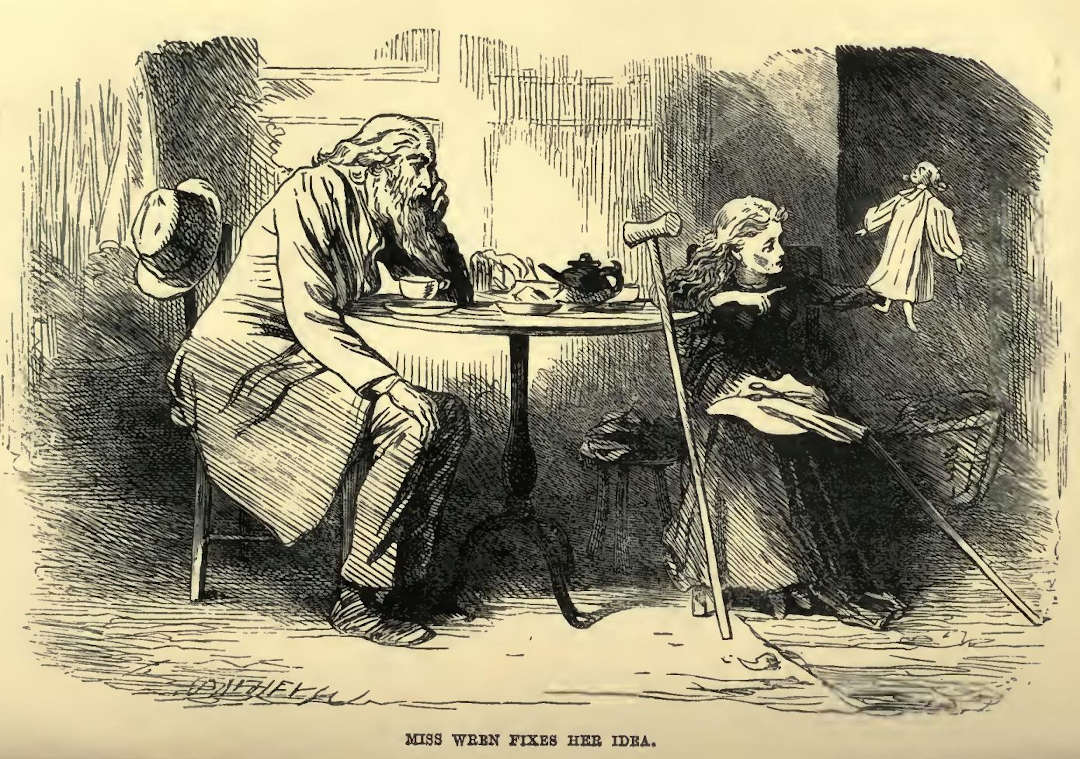
\includegraphics[scale=2.3]{04-09-01}

‘Not a funeral, never fear!’ returned Miss Jenny, anticipating his
objection with a nod. ‘The public don’t like to be made melancholy, I
know very well. I am seldom called upon to put my young friends into
mourning; not into real mourning, that is; Court mourning they are
rather proud of. But a doll clergyman, my dear,--glossy black curls
and whiskers--uniting two of my young friends in matrimony,’ said Miss
Jenny, shaking her forefinger, ‘is quite another affair. If you don’t
see those three at the altar in Bond Street, in a jiffy, my name’s Jack
Robinson!’

With her expert little ways in sharp action, she had got a doll into
whitey-brown paper orders, before the meal was over, and was displaying
it for the edification of the Jewish mind, when a knock was heard at the
street-door. Riah went to open it, and presently came back, ushering in,
with the grave and courteous air that sat so well upon him, a gentleman.

The gentleman was a stranger to the dressmaker; but even in the moment
of his casting his eyes upon her, there was something in his manner
which brought to her remembrance Mr Eugene Wrayburn.

‘Pardon me,’ said the gentleman. ‘You are the dolls’ dressmaker?’

‘I am the dolls’ dressmaker, sir.’

‘Lizzie Hexam’s friend?’

‘Yes, sir,’ replied Miss Jenny, instantly on the defensive. ‘And Lizzie
Hexam’s friend.’

‘Here is a note from her, entreating you to accede to the request of
Mr Mortimer Lightwood, the bearer. Mr Riah chances to know that I am Mr
Mortimer Lightwood, and will tell you so.’

Riah bent his head in corroboration.

‘Will you read the note?’

‘It’s very short,’ said Jenny, with a look of wonder, when she had read
it.

‘There was no time to make it longer. Time was so very precious. My dear
friend Mr Eugene Wrayburn is dying.’

The dressmaker clasped her hands, and uttered a little piteous cry.

‘Is dying,’ repeated Lightwood, with emotion, ‘at some distance from
here. He is sinking under injuries received at the hands of a villain
who attacked him in the dark. I come straight from his bedside. He is
almost always insensible. In a short restless interval of sensibility,
or partial sensibility, I made out that he asked for you to be brought
to sit by him. Hardly relying on my own interpretation of the indistinct
sounds he made, I caused Lizzie to hear them. We were both sure that he
asked for you.’

The dressmaker, with her hands still clasped, looked affrightedly from
the one to the other of her two companions.

‘If you delay, he may die with his request ungratified, with his
last wish--intrusted to me--we have long been much more than
brothers--unfulfilled. I shall break down, if I try to say more.’

In a few moments the black bonnet and the crutch-stick were on duty, the
good Jew was left in possession of the house, and the dolls’ dressmaker,
side by side in a chaise with Mortimer Lightwood, was posting out of
town.



